\documentclass{article}
\usepackage[utf8]{inputenc}
\usepackage{listings}
\usepackage{xcolor}
\usepackage{graphicx, fancyhdr, amsmath, amssymb, amsthm, subfig}
\usepackage{indentfirst}
\usepackage{pdfpages}
\usepackage{dirtree}
\usepackage{lastpage, hyperref, enumerate}
% \usepackage{hyperref, url}

% \pagestyle{fancy}
% \fancyhf{}
% \rhead{Page \thepage\ of \pageref{LastPage}}
\title{Semantic Parsing for First-order Logic}
\author{
	Li Dinghong\\
	Di Wu\\
	Junda Liu\\
	\{lidh1, liujd, wudi\}@shanghaitech.edu.cn
}

\begin{document}
% abstract and beginnings
{
	\newpage
	\maketitle

	\textbf{Abstract} - {In this paper, we present a symbolic model for semantic parsing. Our model takes context-free grammar (CFG) parsing trees as input, and outputs first-order logic (FOL) expressions. We also enforce rules of quantifiers and connectives in FOL, as well as binding and scoping based on properties of CFG parsing trees. Our model resolves binding and scoping within a sentence successfully and is highly generic and reliable. Hopefully, our model can easily be extended to more complex grammars or other languages. }

	\vspace{5pt}
	\textbf{\emph{Keywords:}} {Semantic Parsing, Context-free Grammar, First-order Logic, Parsing Tree, Symbolic Methods}

	\tableofcontents
}

\section{Introduction}{
	\subsection{Background and Motivating Applications}{
		The Goal of semantic parsing is to formalize natural languages. That is, mapping texts in natural languages into formal languges, like first-order logic (FOL) or higher-order logic \cite{artzi}. 

		Semantic parsing can be applied in a wide range of fields both in computer science and outside computer science. Computer security of a software, for instance, cannot be confirmed until it is studied formally and mathematically \cite{avalle}\cite{lal}. Empirical methods like fuzzing are not so reliable because they lack solid foundations \cite{moro}. Thus, semantic parsing is necessary. 

		Formal verification of programming languages \cite{jung} also require to formalize user manuals or official guides, which are typically written in natural languages. Most of these tasks are done by hand now. This is tedious and erroneous. 

		Semantic parsing can also help to prove mathematical theorems as well as to check their proofs automatically. Output of a semantic parser is in logical forms, so it can be accepted by computers \cite{matsuzaki}. Computers can then finish later tasks by inference \cite{chang}. 
	}

	\subsection{Our Contributions}{
		Although supervised learning and neural networks are amazingly successful in natural language processing, advances in semantic parsing are relatively little \cite{reddy}. Most existing methods of semantic parsing are highly restrictive in fields \cite{shi} or grammars. Typically, they can only tackle a very small subset of natural languages, like if-this-then-that structures \cite{quirk} \cite{beltagy}. 

		Thanks to parsing trees, our model is highly generic and rekuabke. We take parsing trees as input instead of original texts so ambiguity of natural languages is not so disturbing. Besides, We can easily reuse it for a different language by simply defining new rules. For instance, we can build a semantic parser for French by adding lexicons and grammars. 

		\cite{matsuzaki} has succeeded to build a semantic parsing framework for pre-university math problems. However, their model fails to determine binding and scoping, since they use dependency trees not CFG. We succeed to build a binding and scoping structures based on CFG parsing trees. 
	}
}

\section{Methods}{
	\subsection{Grammars and Parsing Tree}{
		According to Chomsky hierarchy, formal grammars can be classified as regular grammar, context-free grammar (CFG), context-sensitive grammar and recursively enumerable grammar. 

		Context-sensitive grammar is computationally intractable \cite{lita} and recursively enumerable grammar is even undecideable \cite{merkle}, although they more expressive and more powerful. Besides, regular grammar is obviously too restrictive. Therefore, we can choose either context-free grammar or one of its subsets, dependency grammar \cite{han}. 

		We have first considered dependency grammar, since dependency trees seem to preserve enough information we need. Besides, dependency trees are much smaller than CFG parsing trees. However, we have found it insufficient. Dependency parsing trees cannot provide groups of words within a sentence, but this information is needed for first-order logic. For instance, dependency parsing trees cannot tell scoping of variables explicitly. 

		Therefore, we choose CFG parsing trees as our input. We can get CFG parsing trees from texts in natural languages, and then generate FOL expressions from the trees. 
	}

	\subsection{Recursive Definition of FOL}{
		FOL expressions can be recursively defined in the following way. \cite{andrews}

		Terms can be defined like this: 

		\begin{enumerate}[(a)]
		\item {
			Variables. 
		}

		\item {
			Functions: if $t_1, \cdots, t_n $ are terms, then $f(t_1, \cdots, t_n)$ is a term. 
		}

		\item {
			Constants. 
		}
		\end{enumerate}

		The set of formulas is inductively defined by the following rules:

		\begin{enumerate}[(a)]
		\item {
			Predicate symbols: if $t_1, \cdots, t_n$ are terms then $P(t_1, \cdots, t_n)$ is a formula. 
		}

		\item {
			Equality: if $t_1$ and $t_2$ are terms, then $t_1 = t_2$ is a formula. 
		}

		\item {
			Negation: if $\phi $ is a formula, then $\neg \phi $ is a formula. 
		}

		\item {
			Binary connectives: if $\phi $ and $\varphi $ are formulas, then $\phi B \varphi $ is a formula. 

			$B$ indicates any binary connective. 
		}

		\item {
			Quantifiers: if $\varphi$ is a formula and $x$ is a variable, then $\forall x \varphi$ and $\exists x \varphi $ are formulas.  
		}
		\end{enumerate}

		All FOL expressions are constructed in this way. Therefore, we can also use them to construct FOL expressions from CFG parsing trees. 
	}
}

\section{Parsing Tree Traversal}{
	We develop a symbolic approach for semantic parsing, which is computationally less complex and more reliable and predictable than learning algorithms. We generate first-order logic expressions by traversing CFG parsing trees and defining a small number of rules manually. Since CFG parsing trees are deterministic and informative enough, rules we need to add are very limited. 

	\subsection{Generation of FOL}{
		Now we can generate first-order logic expressions by inductive formation rules. 

		Generation of negation and equality is quite simple. However, generation of binary connectives and quantifiers is not trivial. We have to avoid common mistakes like using $\wedge $ as the main connective with $\forall $, or using $\wedge $ as the main connective with $\Rightarrow $ as the main connective with $\exists $. 

		We thus add some rules to avoid this. Whenever the output expression is started with $\exists $, we have to generate $\wedge $ instead of $\Rightarrow$. 

		Predicate symbols and functions are ubiquitous in first-order logic. To tackle disambiguation as well as binding and scoping more easily, however, we use them even more. We define a new variable name when we meet a constant, and define a constant function for it. 
	}

	\subsection{Binding and Scoping}{
		Binding is not challenging for a single sentence. However, determining scope of variables is not even possible without the help of parsing trees. 

		Our scoping rule is that \textbf{a variable lives within its own constituency within a sentence}. 

		Since CFG parsing trees present information about constituency in a sentence clearly, we can determine the scope of variables easily using CFG parsing trees. 

		For instance, in the sentence "\emph{Some boys in the garden are sad}", units within it are: 

		(Some boys (in (the garden))) (are (sad))

		Define (Some boys (in (the garden))) as $S_1$, (in (the garden)) as $S_2 $, and (the garden) as $S_3 $. 

		If we assign $x$ to \emph{boys}, then the scope of $x$ is $S_1$. Then, we assign $z_2$ to \emph{(the garden)} instead of \emph{garden}. Therefore, the scope of $z_2$ is $S_2 $ instead of $S_3 $. 

		$$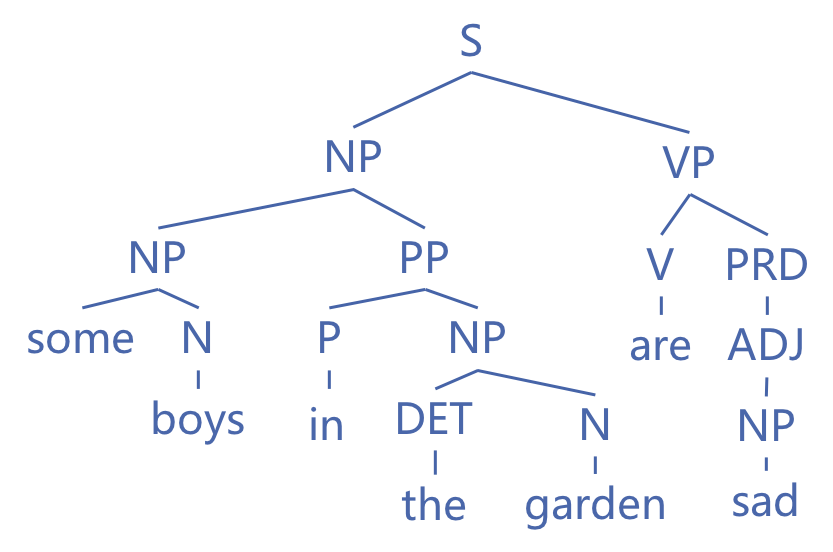
\includegraphics[width = 0.5\textwidth]{tree.png}$$
		\begin{center}
		\small{CFG Parsing Tree of our Example}
		\end{center}
	}
}

\section{Results}{
	We test our model using manually written sentences. Syntax analysis is done by Python package nltk, and the output is CFG parsing trees. 

	Our model can then generate corresponding FOL logic expression correctly for each sentence. That means, our model is reliable for certain types of sentences. 

	Source codes of our work is availabe at \emph{https://github.com/CuthbertLi/Semantic-parsing-logic}. 
}

\section{Conclusion}{
	We succeed to build a generic and reliable model of semantic parsing based on CFG parsing trees. Therefore, symbolic methods are possible to work well for semantic parsing as long as a correct CFG parsing tree is given. A binding and scoping structure based on CFG parsing trees is also introduced in our model. 

	Our future work includes the expansion of the lexicon with the aid of the semantic parser and generalizing our model to other natural languages. 
}

\bibliographystyle{unsrt}
\bibliography{report}
\citation

\end{document}